\documentclass[xcolor=table,xcolor=x11names]{beamer}
\usepackage[utf8]{inputenc}
\usepackage[T1]{fontenc}
\usepackage{booktabs}
\usepackage{makecell}
\usepackage{adjustbox}
\usepackage{graphicx}
\usepackage{subcaption}
\usepackage{pgfplots}

%\usepackage{gnuplot-lua-tikz}
\usepackage{tikz}
\usetikzlibrary{calc,math}
\usetikzlibrary{angles, intersections}






%%%%%%%%%%%%%%%%%%%%%%%%%%%%
%%%% STICKMANS (PELAOs) %%%%
%%%%%%%%%%%%%%%%%%%%%%%%%%%%
\newcommand{\pelao}[3]{% \pelao ==== V
    \draw[
        evaluate={
            \x = (#1); % center x
            \y = (#2); % center y
            \r = (#3); % radius
            \xl = \x-\r; % x left
            \xr = \x+\r; % x right
            \ya = \y-\r; % body upper
            \yb = \ya-.75*\r; % arms
            \yc = \yb-\r; % legs
            \ybd = \yb-0*\r; % arms lower
            \ycd = \yc-0.75*\r; % legs lower
        }% ,thin
    ]
    (\x, \y) circle (\r) % head
    (\x, \ya) -- (\x,\yc) % body
    (\xl, \ybd) -- (\x, \yb) -- (\xr, \ybd) %arms
    (\xl, \ycd) -- (\x, \yc) -- (\xr, \ycd) %arms
    ; %
} % \pelao ==== A

%%%%%%%%%%%%%%%%%%%%%%%%%%%%%%%%%%%%
%%%% RUNNING STICKMANS (PELAOs) %%%%
%%%%%%%%%%%%%%%%%%%%%%%%%%%%%%%%%%%%
\newcommand{\runpelao}[4]{% \pelao ==== V
    \draw[
        rotate around={(#4):((#1,#2))},
        evaluate={
            \xn = (#1); % center xn
            \yn = (#2); % center yn
            \r = (#3); % radius
            \xnl = \xn-\r; % xn left
            \xnr = \xn+\r; % xn right
            \yna = \yn-\r; % bodyn upper
            \ynb = \yna-.75*\r; % arms
            \ync = \ynb-\r; % legs
            \ynbd = \ynb-0*\r; % arms lower
            \yncd = \ync-0.75*\r; % legs lower
        }% ,thin
    ]
    (\xn, \yn) circle (\r) % head
    (\xn, \yna) -- (\xn,\ync) % bodyn
    (\xnl, \ynbd) -- (\xn, \ynb) -- (\xnr, \ynbd) %arms
    (\xnl, \yncd) -- (\xn, \ync) -- (\xnr, \yncd) %arms
    (\xnr, \ynbd) -- (\xnr, \ynbd+.1) %hands
    (\xnl, \ynbd) -- (\xnl, \ynbd-.1) %hands
    ; %
} % \pelao ==== A






\title{NR sensing testbed \& Semantic Compression}
\date{13 de marzo de 2025}
\author{Pablo Fernández López\\Jorge Martín Pérez}

\usepackage[spanish]{babel}

\usetheme[girosiptc]{upm}



\AtBeginSection[]
{
  \begin{frame}{Table of Contents}
    \tableofcontents[currentsection]
  \end{frame}
}



\begin{document}


\begin{frame}
\titlepage
\end{frame}


\begin{frame}{Table of Contents}
    \tableofcontents
\end{frame}

\setcounter{framenumber}{0}



\section{Semantic Encoding}


\begin{frame}{\secname}
    \begin{figure}
        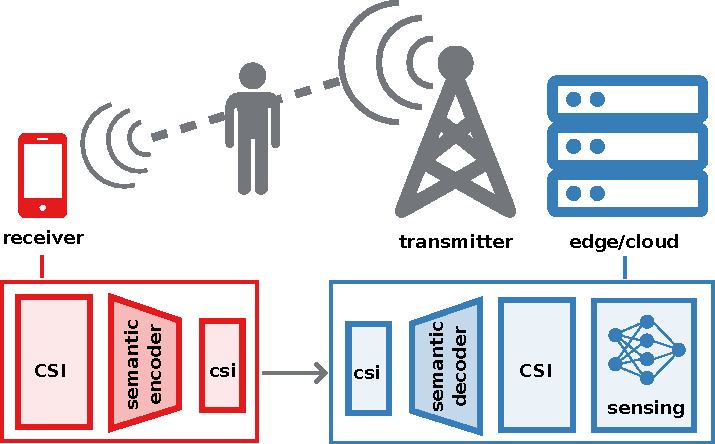
\includegraphics[width=.8\textwidth]{figures/front}
        \caption{The 5G CSI is compressed through a semantic
        encoder. The encoded CSI is decoded and processed
        at the edge/cloud for sensing purposes.}
    \end{figure}
\end{frame}


\begin{frame}{\secname}
    Semantic communications:
    \begin{quote}
        transmit necessary information relevant to the specific task
    \end{quote}
    that we want to perform:
    \pause
    {\color{blue}sensing!}
    \pause
    \vfill
    \begin{figure}
        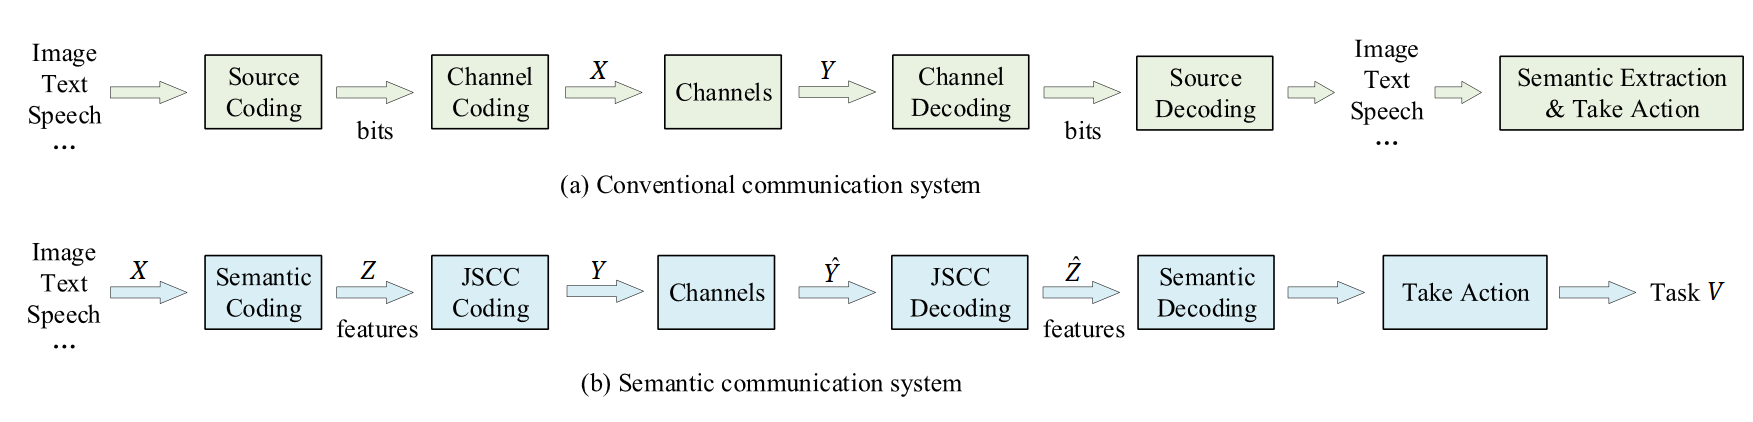
\includegraphics[width=\textwidth]{figures/semantic}
        \caption{arXiv 2201.01389}
    \end{figure}
\end{frame}



\begin{frame}{\secname}
    What is the SoA doing?
    \begin{itemize}
        \item Semantic Encoders: VAE, codebooks, detection on latent space
        \item Joint Source Channel Coding as DeepJSCC
    \end{itemize}

    \pause

    \vfill
    The {\color{red}pitfall}:
    \begin{itemize}
        \item fixed codebooks/compression rates of size $K$
        \item different NN architectures per compression size $K$
        \item retrain for each compression size $K$
        \item sensing detectors retraining for each compression size $K$
    \end{itemize}
\end{frame}




\begin{frame}{\secname}
    What do we propose?
    \begin{itemize}
        \item semantic encoder with {\color{blue}\emph{on the fly}}
            compression rate $K$
        \item segment the grid
        \item maximum compression outside the SSB
        \item {\color{blue}reuse} pre-trained sensing detectors
    \end{itemize}

    \begin{figure}
        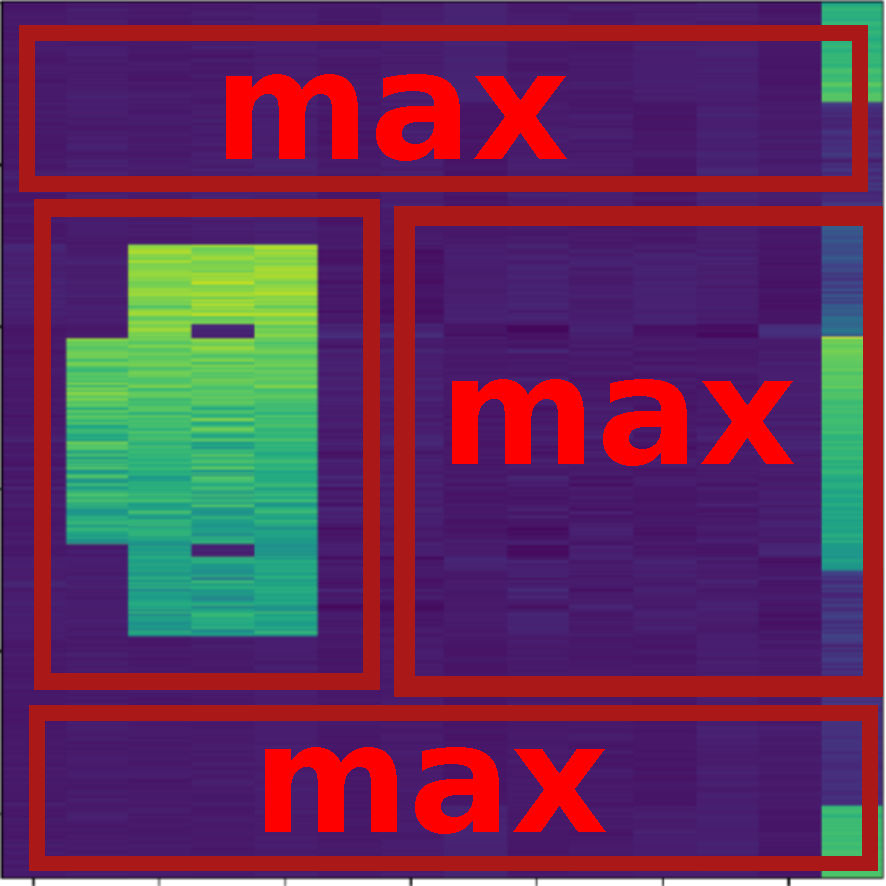
\includegraphics[width=.35\textwidth]{figures/max-compression}
        \caption{}
    \end{figure}
\end{frame}



\begin{frame}{\secname}

    Metric for the semantic similarity: Wasserstrein distance.\\
    {\color{blue}Experiment}: compression impact on sensing accuracy
    @12k grids

    \pause

    \begin{columns}
% Column 1
% Column 2
    \begin{column}{.5\textwidth}
    \begin{figure}
        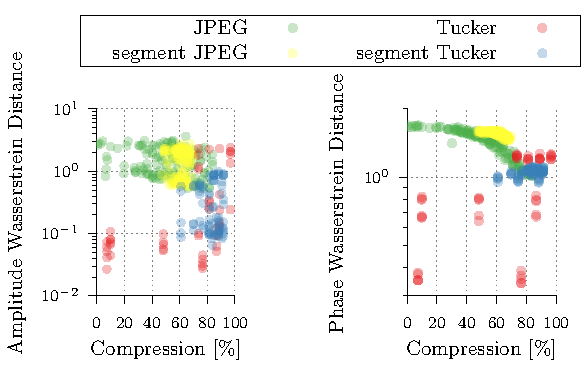
\includegraphics[width=\textwidth]{figures/wasserstrein-standalone}
        \caption{}
    \end{figure}
    \end{column}%
    \begin{column}{.5\textwidth}
    \begin{figure}
        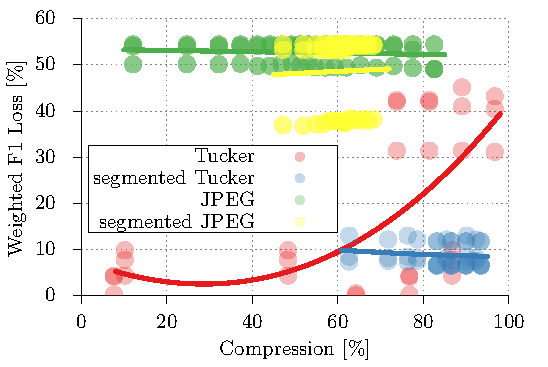
\includegraphics[width=\textwidth]{figures/o-standalone}
        \caption{}
    \end{figure}
    \end{column}

\end{columns}

    \pause

{\color{blue}Take-aways}:
\begin{itemize}
    \item more compression doesn't mean more loss
    \item segmented encoding/compression achieves
        ($i$) higher compression; and
        ($ii$) better accuracy.
\end{itemize}

\end{frame}




\section{NR sensing testbed}
\begin{frame}{\secname}
    Tasks done:
    \begin{itemize}
        \item Implemented a person detection script based on \href{https://docs.ultralytics.com/}{\textit{Ultralytics YOLO}} to log human presence.
        \item Implemented relative depth detection with \href{https://github.com/DepthAnything/Depth-Anything-V2}{\textit{Depth Anything V2}}.
        \item Conducted preliminary tests in the selected emplacement for the capture campaign.
    \end{itemize}
\end{frame}

\begin{frame}{\secname}
    Person and depth detection for automatic tagging of the data set.
    \begin{figure}
        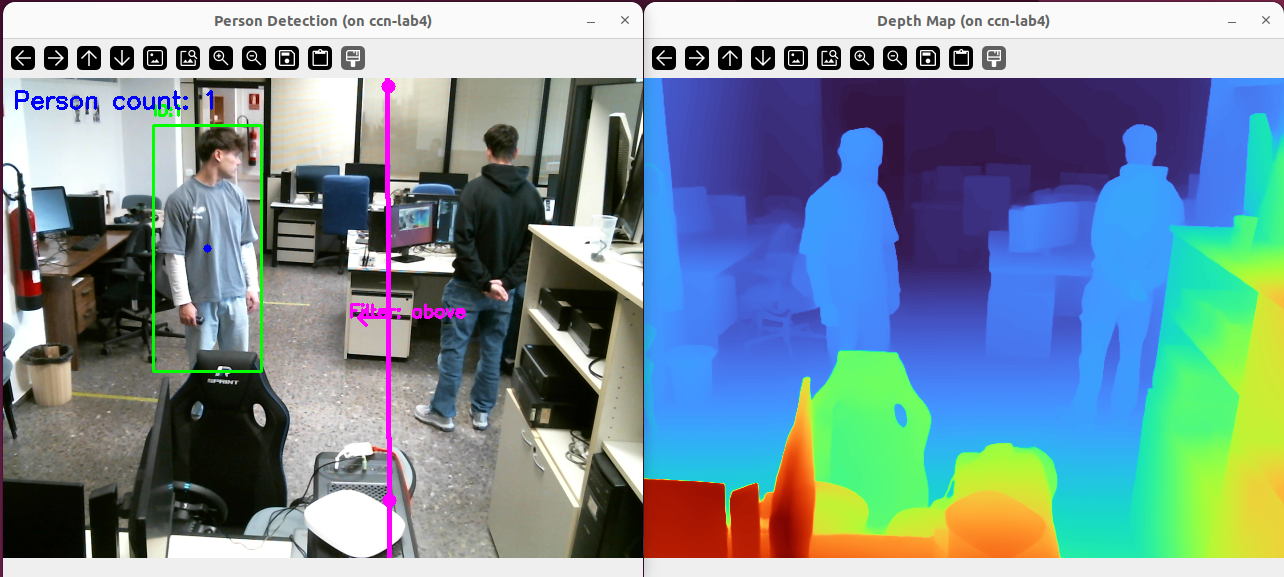
\includegraphics[width=.8\textwidth]{figures/YOLO_detect1.png}
        \caption{One person detected within virtual boundary}
    \end{figure}
\end{frame}

\begin{frame}{\secname}
    Person and depth detection for automatic tagging of the data set.
    \begin{figure}
        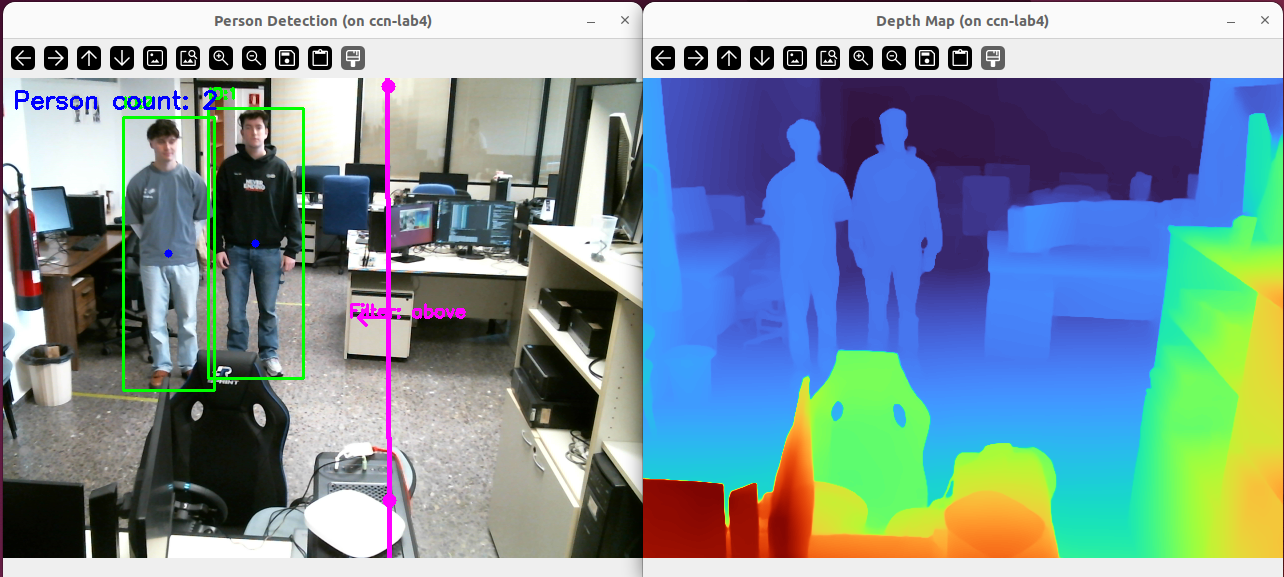
\includegraphics[width=.8\textwidth]{figures/YOLO_detect2.png}
        \caption{Two people detected within virtual boundary}
    \end{figure}
\end{frame}

\begin{frame}{\secname}
    Pending tasks:
    \begin{itemize}
        \item Implementation, training, and testing of state-of-the-art CNN architectures for presence detection.
        \item Inference testing with compressed resource grids.
        \item Capture of a large real scenario dataset.
    \end{itemize}
\end{frame}

\section{Semantic Compression}
\begin{frame}{\secname}
    After modulation the NR grid is decomposed
    in amplitude \& phase @each RB.
    \begin{figure}
        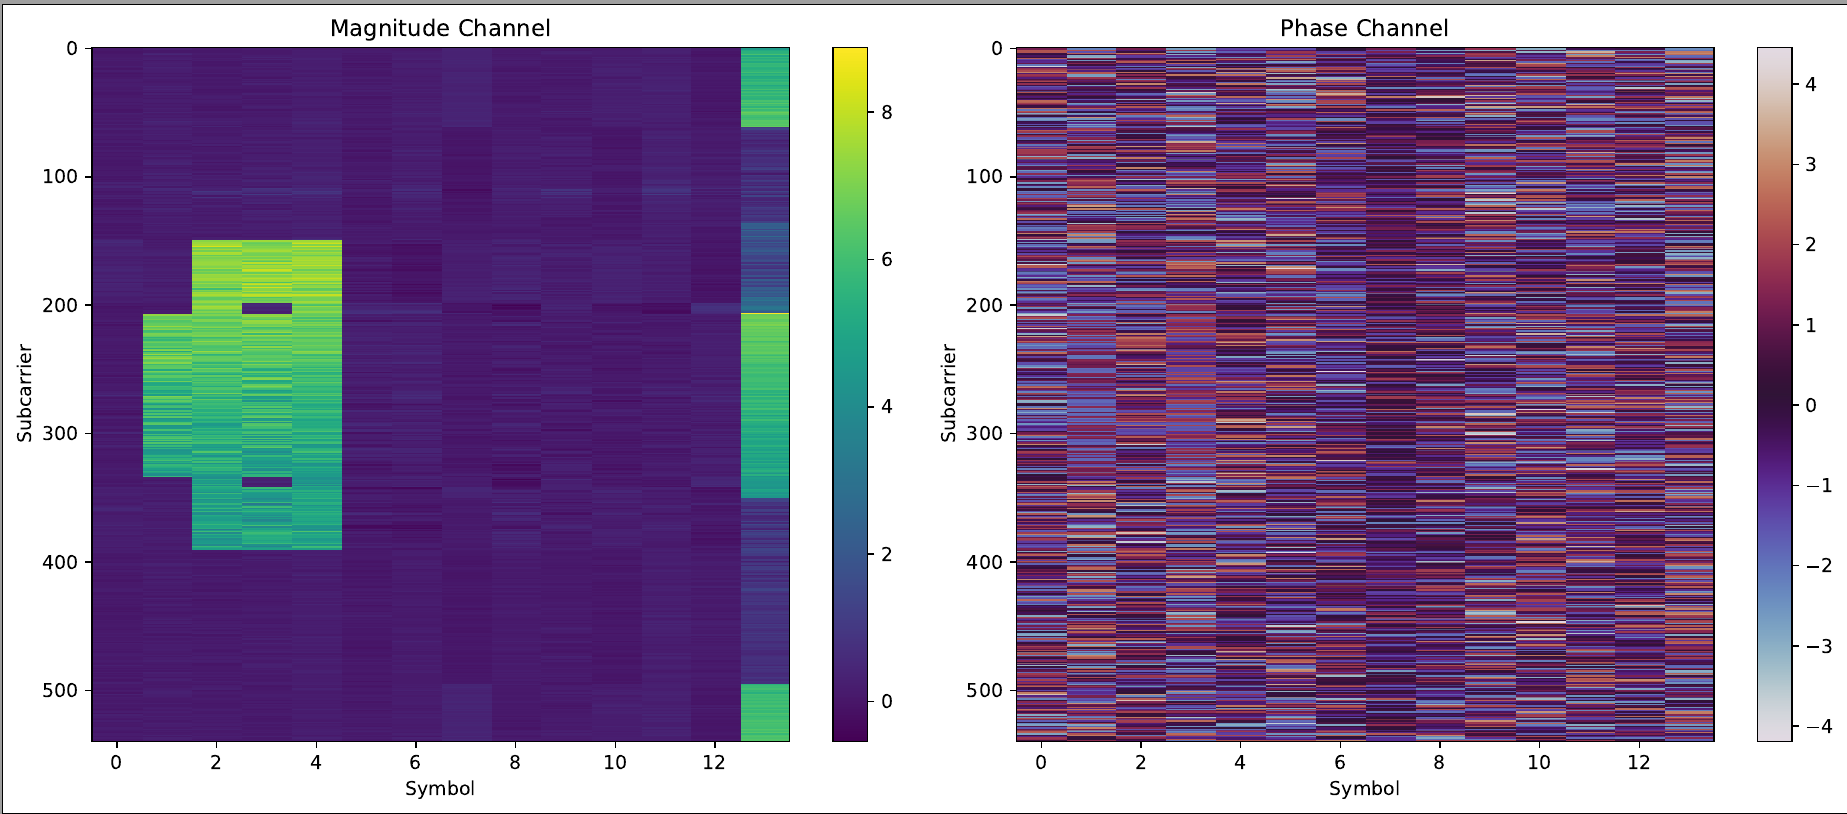
\includegraphics[width=.8\textwidth]{figures/grid.png}
        \caption{}
    \end{figure}
    The testbed captures SSBs.
\end{frame}

\begin{frame}{\secname}
    \emph{Task}: perform AI sensing inference @cloud

    \pause
    \emph{Problem}: each UE exchanges {\color{red}46\,\textrm{Mbps}} using
    \texttt{torch.float64}

    \pause
    \emph{Solutions}: to reduce the bandwidth:
    \begin{itemize}
        \item use \texttt{torch.float32}, \texttt{torch.float16}, etc.; or
        \item {\color{olive}compress} the NR grid.
    \end{itemize}
\end{frame}


\begin{frame}{\secname: compression techniques}
    We try the following compressions on the NR
    tensors {\color{olive}\texttt{grid.pt}}:
    \begin{itemize}
        \item Lossless
            \begin{itemize}
                \item \textbf{ZIP} with a 10\% compression
                \item \textbf{LZ4} with a 6\% compression
            \end{itemize}
        \item Lossy
            \begin{itemize}
                \item \textbf{JPEG} up to a {\color{olive}98\%} compression
                \item \textbf{JSCC} also $\sim$99\% compression 
                \item \textbf{CP} just a $\sim50\%$ compression
                \item \textbf{Tucker} up to a {\color{olive}99.44\%} compression
            \end{itemize}
    \end{itemize}
\end{frame}


\begin{frame}{\secname: JPEG}
    We perform compression separately on amplitude/phase channels.

    \begin{figure}
        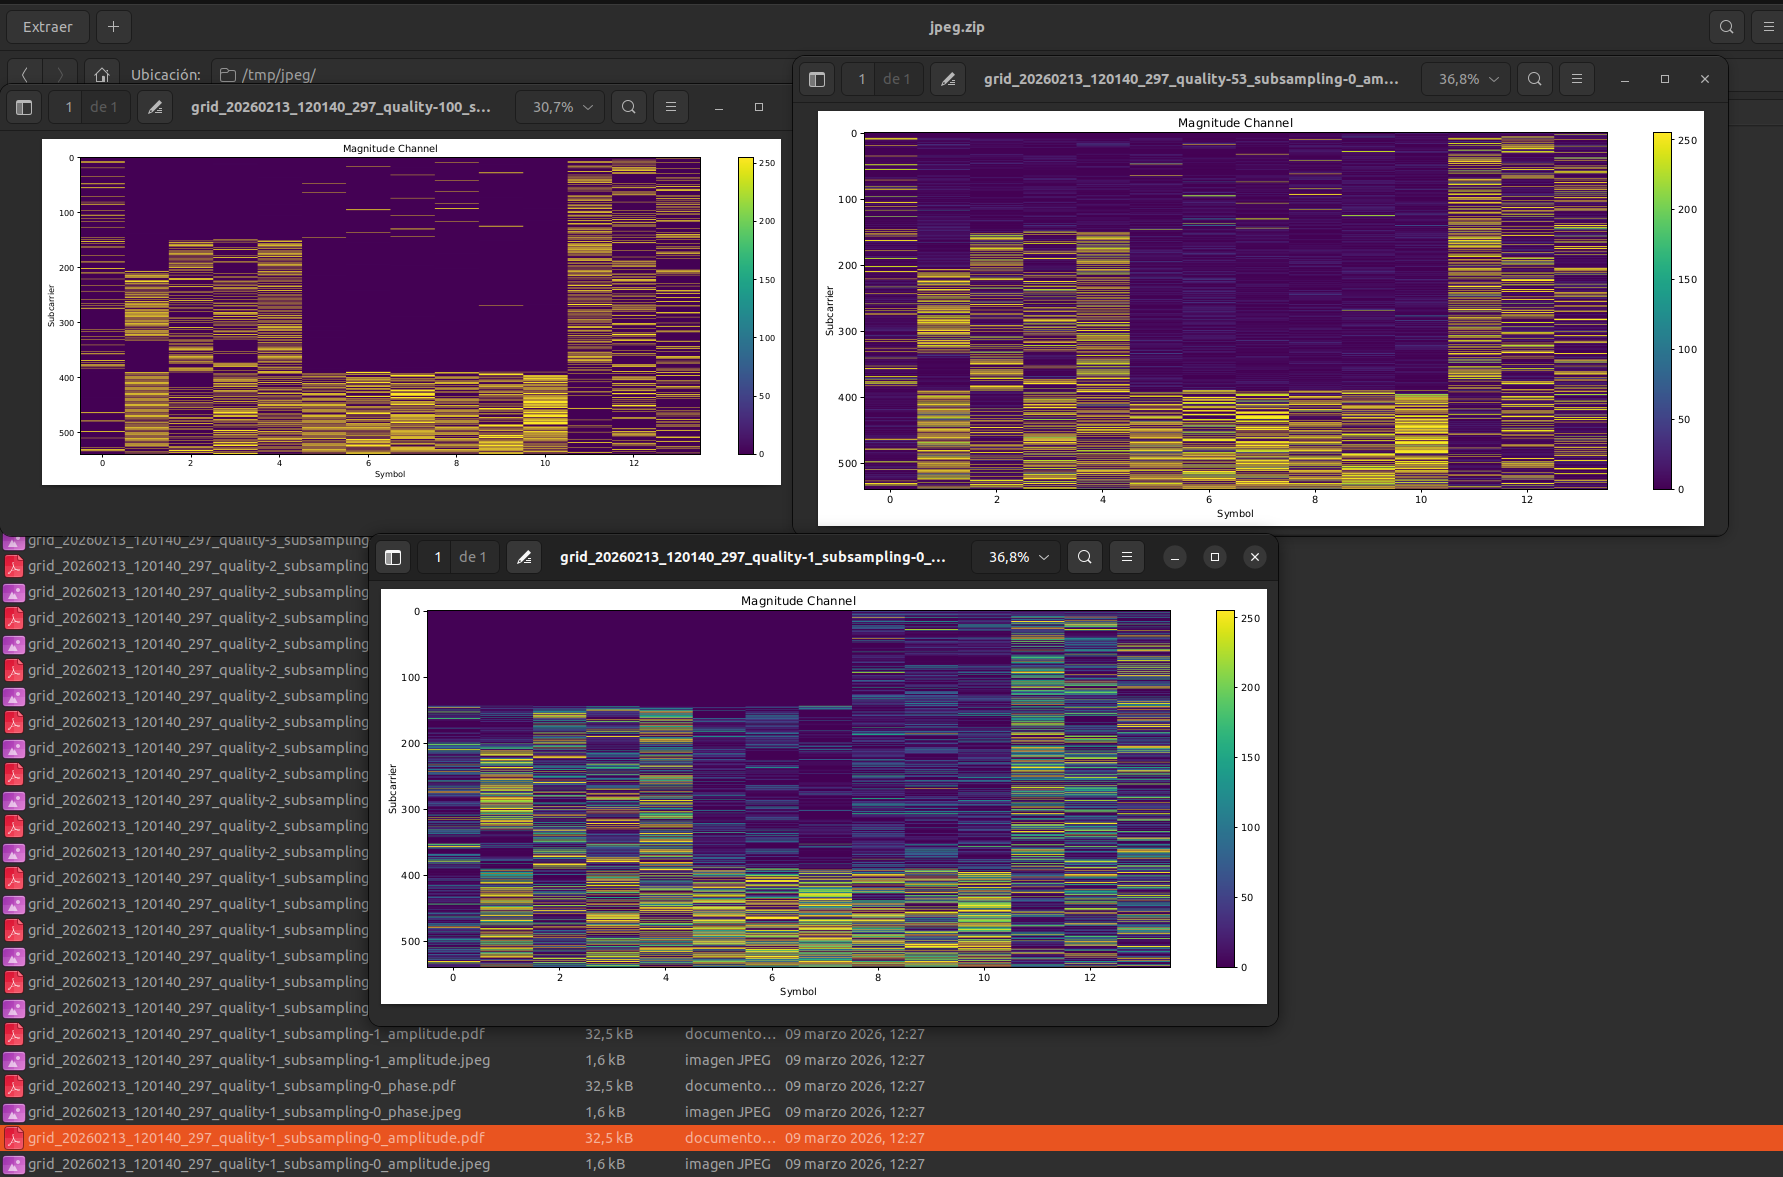
\includegraphics[width=.8\textwidth]{figures/jpeg.png}
        \caption{100, 50, and 1 JPEG quality}
    \end{figure}
\end{frame}




\begin{frame}{\secname: Tucker decomposition}
    Original {\color{olive}NR grid}
    tensor ${\color{olive}T} \in F^{n_{1} \times n_{2} \times n_{3}}$
    decomposed as
    \begin{equation}
        {\color{olive}T} = {\color{blue}\mathcal{T}} \times_{1} U^{(1)} \times_{2} U^{(2)} \times_{3} U^{(3)}
    \end{equation}
    with ${\color{blue}\mathcal{T}} \in F^{d_{1} \times d_{2} \times d_{3}}$
    the compressed tensor, and the $k$-mode products:
    \begin{align}
(\mathcal{T} \times_{1} U^{(1)})(i_{1}, j_{2}, j_{3}) &= \sum_{j_{1}=1}^{d_{1}} \mathcal{T}(j_{1}, j_{2}, j_{3})U^{(1)}(j_{1}, i_{1}) \\
(\mathcal{T} \times_{2} U^{(2)})(j_{1}, i_{2}, j_{3}) &= \sum_{j_{2}=1}^{d_{2}} \mathcal{T}(j_{1}, j_{2}, j_{3})U^{(2)}(j_{2}, i_{2}) \\
(\mathcal{T} \times_{3} U^{(3)})(j_{1}, j_{2}, i_{3}) &= \sum_{j_{3}=1}^{d_{3}} \mathcal{T}(j_{1}, j_{2}, j_{3})U^{(3)}(j_{3}, i_{3})
\end{align}

\end{frame}


\begin{frame}{\secname: Tucker decomposition}
    \begin{figure}
        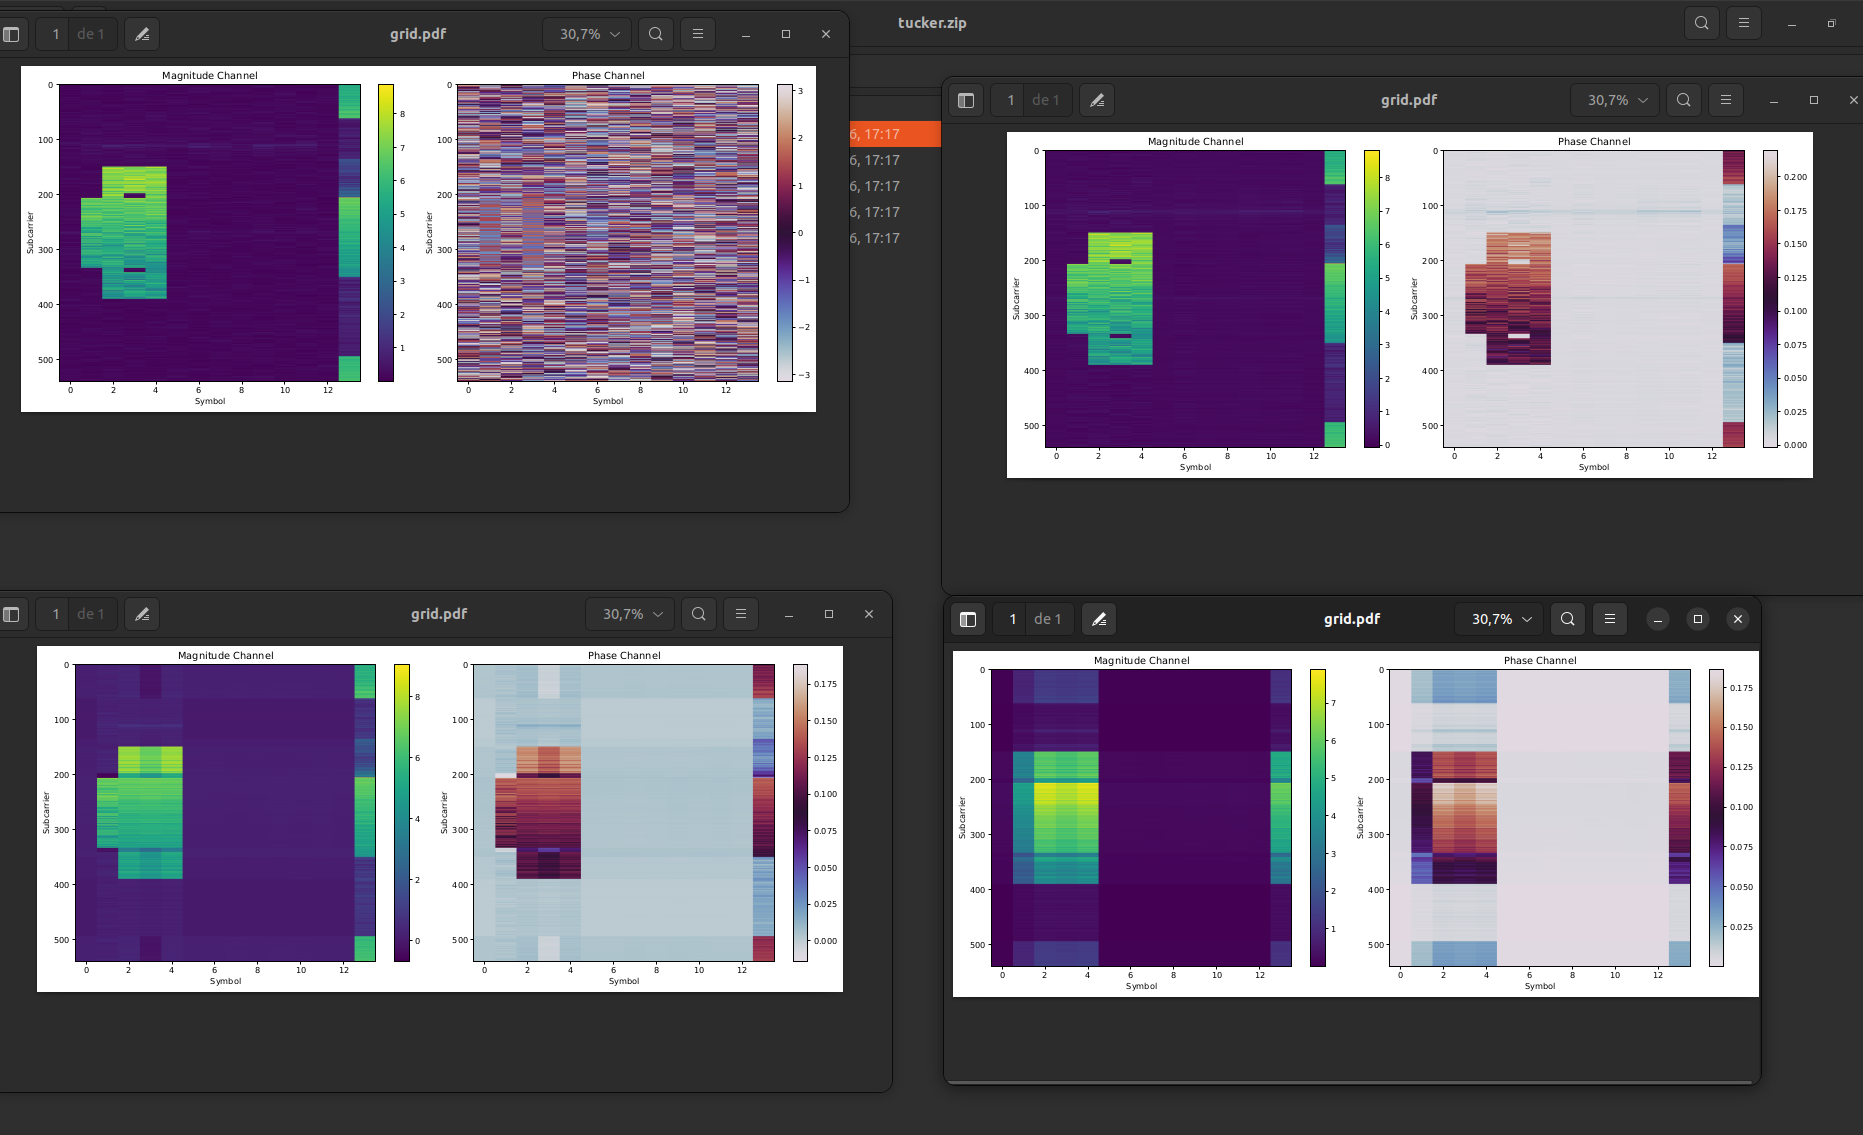
\includegraphics[width=.8\textwidth]{figures/tucker.png}
        \caption{Tucker with $d_1=2$, 0,50,75,100\% compression.}
    \end{figure}

\end{frame}



\begin{frame}{\secname: Tucker decomposition}
    \begin{figure}
        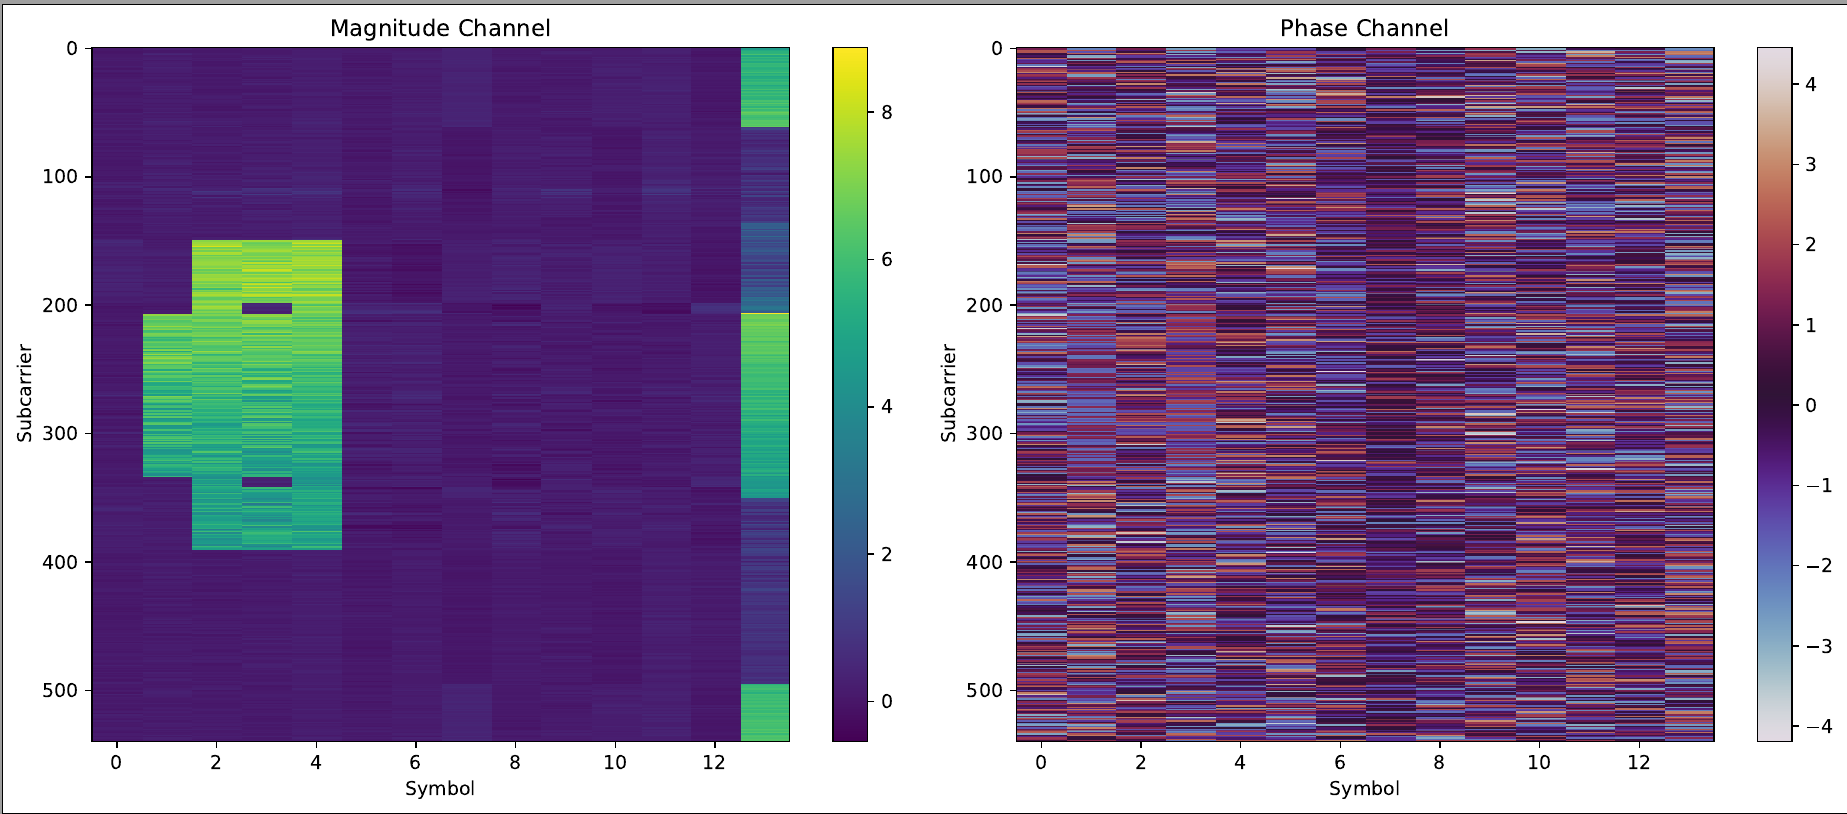
\includegraphics[width=.8\textwidth]{figures/tucker2.png}
        \caption{Tucker with $d_1=1$ and 50\% compression.}
    \end{figure}
\end{frame}



\begin{frame}{\secname: next steps}
    \begin{itemize}
        \item Apply semantic segmentation and compression:
            \begin{itemize}
                \item Compress SSB
                \item Compress x4 regions arround SSB
            \end{itemize}
        \item Assess AI/ML sensing detectors performance with
            compressed NR grids
    \end{itemize}
\end{frame}



\end{document}
